\section{Numerical}

In this section, numerical experiments will be conducted to test the developed method,
and to evaluate wether it can be deployed in a real scenario.

The experiment will proceed in the following way:
in the first place, a profile for a theoretical travel time function will be defined.
This profile will need to satisfy assumptions NUMBERS\todo{Cite all the assumptions},
in order to be similar to a profile that could be found in reality.

After the function has been defined,
shapes for the distributions of the parameters \(B, \Gamma, T^*\) will be fixed,
dependant on a parameter \(\theta \in \R^d\).

Given all of this and a value \(\theta_0\) for the shape parameter \(\theta\),
a dataset of synthetic observations can be built accordingly to the model.
The dataset is constructed by sampling the parameters \(\beta, \gamma, t^*\) and explicitly minimizing the resulting cost function.
This yields a dataset for which the real value of the parameter \(\theta\),
which affects the distributions of \(B, \Gamma, T^*\), is known,
allowing the actual convergence of the estimation to be evaluated in a simple scenario,
and the behaviour of the likelihood function to be shown when the dataset is fixed.

\subsection{Choosing the parameters}

As explained above,
the first step to be done consists in choosing the travel time function and the distributions of the parameters.

\subsubsection{Travel Time Function}

The travel time function must be chosen accordingly to assumptions \todo{What assumptions?}:
it hence has to be continuous and with continuous derivative,
and its derivative upper bounded by \(1\).
Moreover, it has to satisfy assumption \todo{assumption number},
that defines when the function is concave and when convex.

A gaussian function satisfies all the assumptions,
as long as its variance is high enough.
For better capturing the expected asymmetricity for early and late arrivals,
two different variances will be considered before and after the peak.
The considered function will thus be
\begin{equation}
  \label{eq:tt_def}
  tt(t) =
  \begin{cases}
    e^{-\frac{(x - \mu)^2}{\sigma_l}} & \text{if } x \leq \mu \\
    e^{-\frac{(x - \mu)^2}{\sigma_r}} & \text{if } x > \mu
  \end{cases}
\end{equation}

The resulting function is shown in figure\todo{Put figure}.
It satisfies assumption NUMBER\todo{put number},
since
\begin{equation*}
  \lim_{t \rightarrow 0}tt'(t) = 0.
\end{equation*}
Moreover, by setting an high enough value for the parameter \(\sigma_l\),
determining the variance for the left part of the function,
assumption NUMBER\todo{put number} is satisfied as well.

A distribution for the random variables \(B, \Gamma, T^*\) has now to be assumed.

\subsubsection{Parameters Distributions}

For simplicity, we consider the parameters to be normally distributed:
\begin{align}
  \label{eq:par-distr}
  B \sim \mathcal{N}(\mu_\beta, \sigma) && \Gamma \sim \mathcal{N}(\mu_\gamma, \sigma) && T^* \sim \mathcal{N}(\mu_t, \sigma_t)
\end{align}

The parameters \(B, \Gamma\) are assumed to have the same variance for reducing the parameter space dimensionality when doing the estimation.

Note that, in case the parameters are assumed to be bounded
(for instance, values of \(\beta, \gamma < 0\) can be excluded),
the distributions can be truncated where needed.

This choice of the distributions will induce a choice of the parameter \(\theta\),
the vector of all the parameters appearing in expression~\eqref{eq:par-distr}.
It will thus be defined as
\begin{equation*}
  \theta =
  \begin{pmatrix}
    \mu_\beta \\
    \mu_\gamma \\
    \mu_t \\
    \sigma \\
    \sigma_t
  \end{pmatrix}
  \in \R^5
\end{equation*}

\subsection{Synthetic Dataset}

For creating the synthetic dataset,
the cost function must be explicitly minimized,
with parameters sampled accordingly to the distributions of the random variables \(B, \Gamma, T^*\).

At first, the size of the synthetic dataset \(N\) is fixed.
\(N\) realizations of the random variables \(B, \Gamma, T^*\) are then sampled from the distributions,
yielding a dataset of triples
\begin{equation*}
  \{\beta_i, \gamma_i, t^*_i\}_i
\end{equation*}

By minimizing the cost function with each one of this triples we are able to generate the dataset of arrival times:

\begin{equation*}
  t_i = \argmin_t C(t; \beta_i, \gamma_i, t^*_i)
\end{equation*}

The minimization is done by explicitly finding the (at most) two internal minima,
which correspond to early and late arrivals,
without relying on the theory built in section NUMBER\todo{put number}
(since relying on the model itself is to be avoided when a model is being validated).

The values found in this way are then compared with the only discontinuity of the derivative,
that is, for \(t = t^*\).
The global minimum for the cost function is thus found in this way.

For finding the finding the time values corresponding to the internal minima,
two gradient descent algorithms are used:
one of them, converging to the late minimum,
will be initialized at a time point that is unlikely to be before any late arrival time (e. g. \(t = 24\)),
while the other one will be initialized at a time point unlikely to be after any early arrival time (e. g. \(t = 0\)).
Since the function is close to linear until the minima occur,
no acceleration technique is used,
as the step size could become greater than needed,
preventing the algorithms from converging at the desired minimum.

\begin{figure}
  \centering
  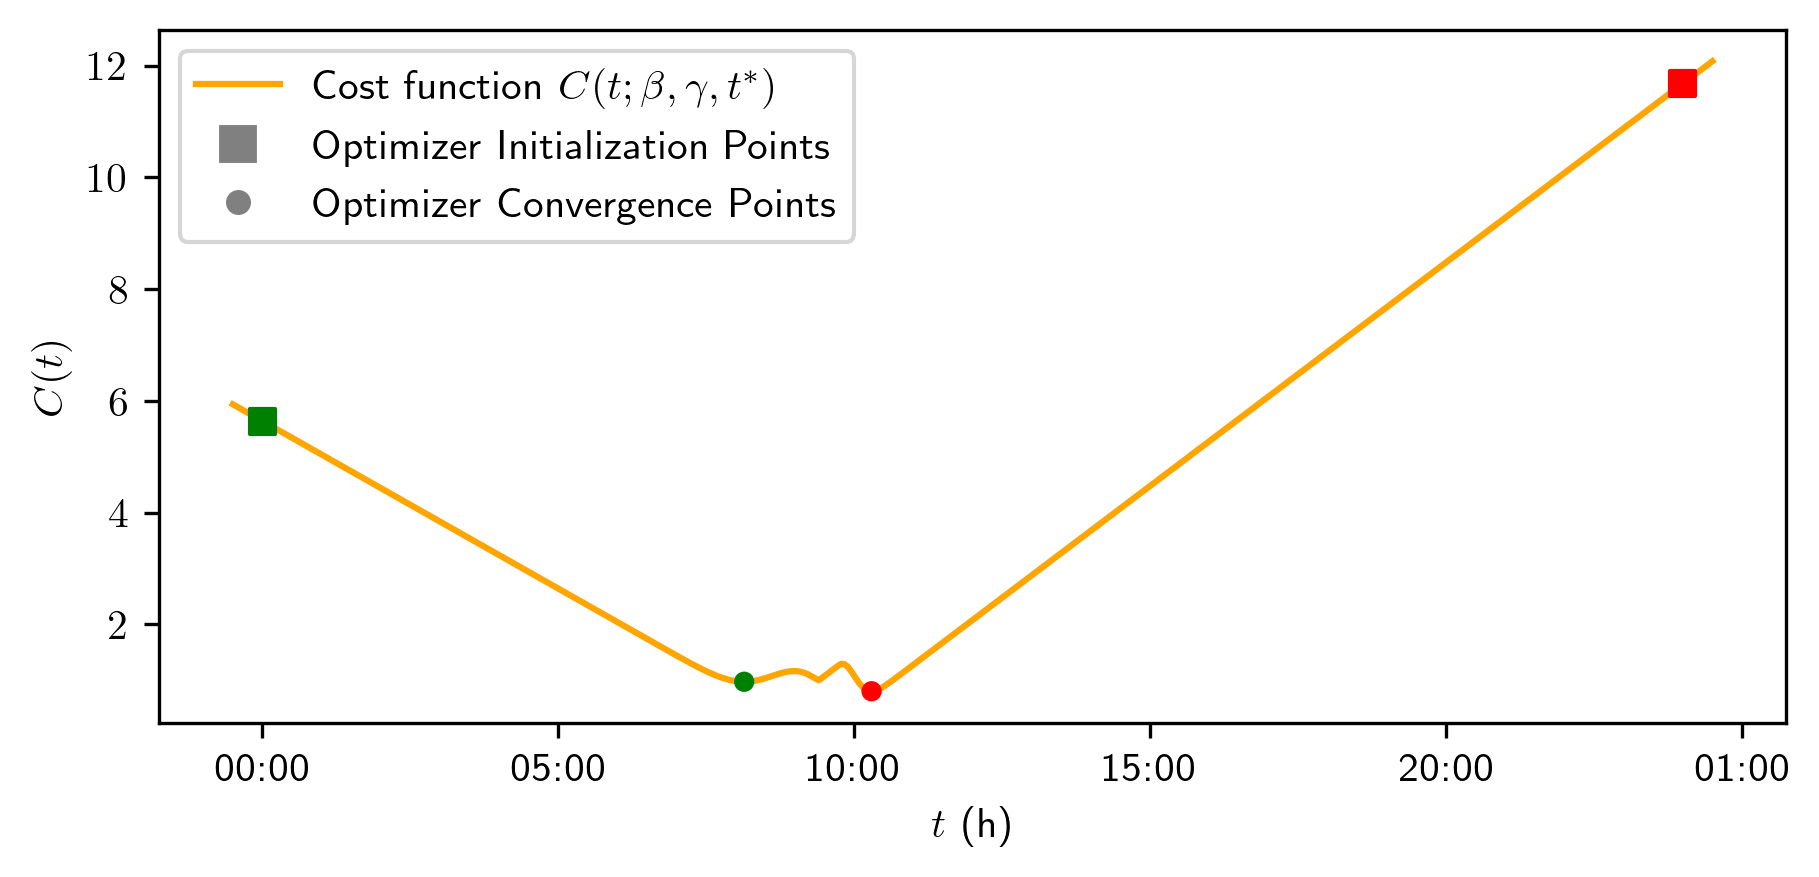
\includegraphics[width=.8\textwidth]{optimizer_cost}
  \caption{
    Cost function,
    plotted with points corresponding to the optimizers initializations and the minima at which they converge.
    The optimizer in green converges to the early minimum,
    while the one in red converges to the late minimum.
    Comparing the found minima with the cost of arriving on-time the minimizer of the cost is found.
    Parameter values used for this cost function are \(\beta = 0.6, \gamma = 0.8\).
  }
  \label{fig:optimizer-cost}
\end{figure}

Figure~\ref{fig:optimizer-cost} shows the cost function,
and depicts how the optimization process is performed.

Figure NUMBER shows distribution,
figure NUMBER overlap likelihood,
please note that is good.\todo{complete these sentences}

%%% Local Variables:
%%% mode: LaTeX
%%% TeX-master: "../main"
%%% End:
